\section{GitOps}

The concept of GitOps enforces using Git as \emph{single source of truth defining the application state.}

Instead of different people using \emph{kubectl create / apply} or \emph{helm install / upgrade} commands from their own laptops, 
the whole configuration of a kubernetes cluster is kept inside a (separate!) Git repository.

This brings the known advantages of a version control system to Continuous Delivery for Kubernetes Clusters:

\begin{itemize}
    \item \textbf{Versioned and immutable}
    \item \textbf{Declarative} definitions of apps, environments and configurations
    \item \textbf{Automated and repeatable}, less opportunity for errors
    \item Code review for changes
    \item Tracking of who did what
    \item Rollback via Git
    \item Whole infrastructure can be recreated from source control
\end{itemize}

Separating the git repository holding kubernetes manifests and the actual application code provides more simplicity when updating some deployment information.

No build and test pipeline will be triggered without any change to the actual code.
Git history will be cleaner.
Application may be distributed over several git repositories.
Separation of access is possible.

\subsection{ArgoCD}
Declarative GitOps tool used to deploy applications on Kubernetes. 

It is lightweight, easy to configure, built with GitOps Workflow in mind and intended only for Kubernetes.

\begin{figure}[h]
    \centering
    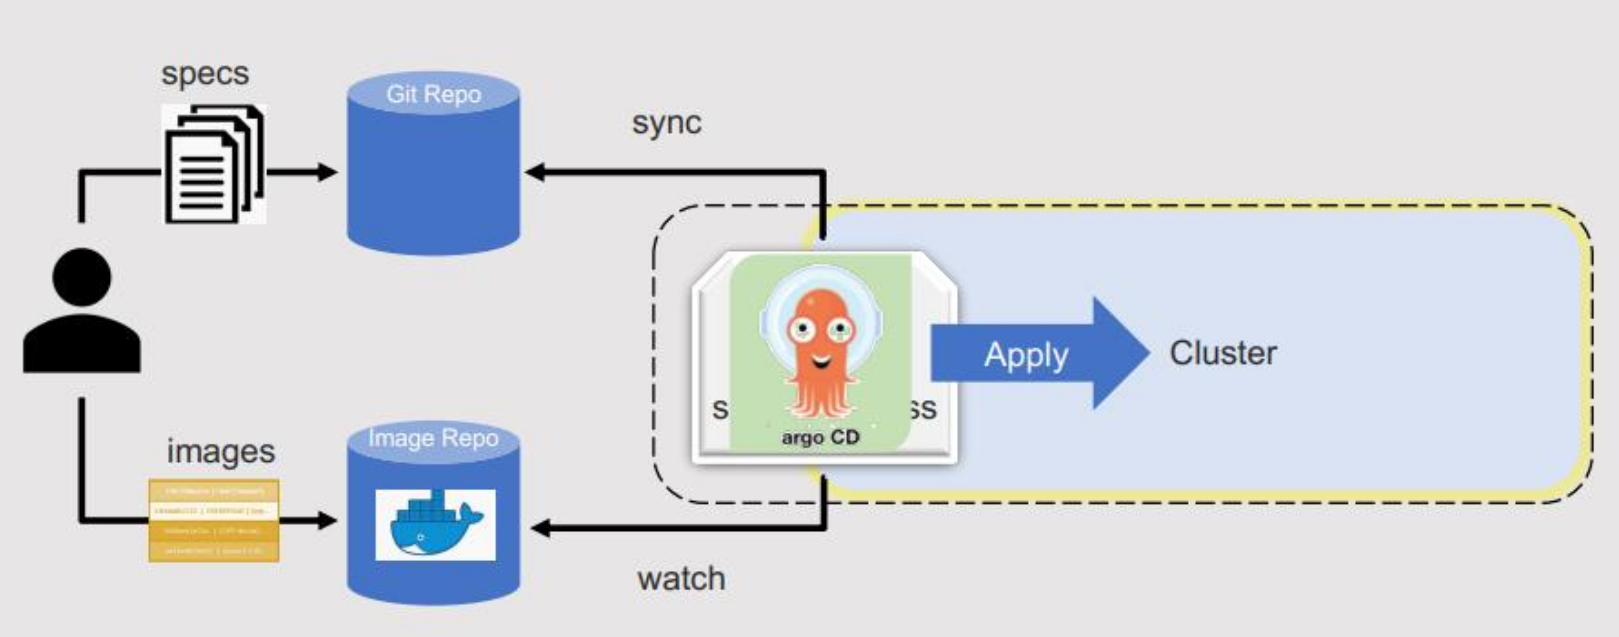
\includegraphics[width=\textwidth]{gitops-argocd}
\end{figure}

\noindent
How does it work?
\begin{itemize}
    \item Spins up its own controller inside the cluster
    \item watches for changes in a repository
    \item compares against resources deployed in the cluster
    \item synchronizes both states (desired state wins)
\end{itemize}

\noindent
Its key concepts are the following:
\renewcommand{\arraystretch}{1.5}
\begin{center}
    \begin{tabular}{p{0.25\textwidth}|p{0.75\textwidth}}
        App/Application & Group of K8s resources defined by a manifest (CRD), used to monitor repository and update cluster \\
        \hline
        Application source type & Which build tool is used to build the app \\
        \hline
        Live State & Current state of the application cluster \\
        \hline
        Target State & Desired state as stored in Git \\
        \hline
        Sync Status & Is live the same as target? \\ 
        \hline
        Sync & Updating app to the target state \\
        \hline
        Sync operation 
        
        status & Success/failure state of the sync operation \\
        \hline
        Refresh & Comparison of Code in Git with live state (.. of Sync Status) \\
        \hline
        Health Status & Is the app running correctly? Serving Requests? \\
        \hline
        Configuration
        
        Management Tool & Tool to create manifests from files in direcory (Kustomize, Ksonnet) \\
        \hline
        Configuration Management Plugin &  Custom tools \ldots \\
    \end{tabular}
\end{center}

\subsection{ArgoCD Application}
Specifies information such as ArgoCD project, source repo, revision, path, cluster, namespace.

Can be created via command line, Web Interface, Yaml in web, K8s Manifest (CRD).

Can be specified using kustomize, helm, ksonnet, jsonnet, plain yaml, custom configuration management tool set up as plugin to ArgoCD.

\vspace{3mm}
\ttfamily argocd app create, argocd list 
\rmfamily

\vspace{3mm}
\noindent
Different app health statuses include 
\begin{itemize}
    \item Progressing
    \item healthy
    \item Degraded
    \item Suspended
    \item Missing
\end{itemize}

\subsubsection{History and Rollback}
ArgoCD keeps track of the various versions deployed and allows you to go back to a previous state.
Can be accessed from the graphical user interface.

\subsubsection{Manual Sync}
\begin{itemize}
    \item \textbf{Prune}: Allow deleting resources that are unexpected, meaning they no longer exist in git.
    \item \textbf{Dry Run}: Preview what an apply operation would do without affecting the cluster
    \item \textbf{Apply only}: Skip pre/post sync hooks
    \item \textbf{Force}: Deletes and re-creates resource(s) when patch encounters conflict after 5 retries 
\end{itemize}

\subsubsection{Automated Sync}
Only occurs if App Sync Status is \emph{OutOfSync}. Attempts one sync per unique combination of commit hash and parameters of the app -- unless \emph{selfHeal} flag is true.

\emph{sefHeal} attempts to sync after a default timeout of 5 seconds. 

\subsubsection{ArgoCD Projects}
Projects can be a logical group of applications, which supports organization by teams.

Features include restrictions and roles to isolate different teams and the resources available inside a project.

\begin{figure}[h]
    \centering
    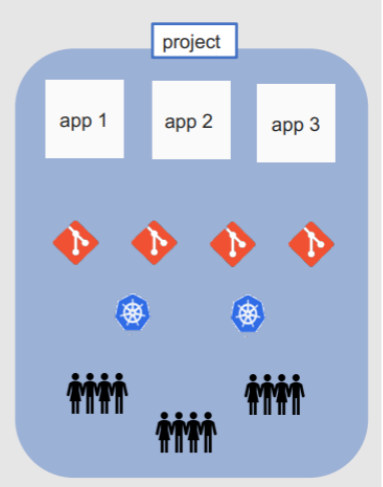
\includegraphics[width=7cm]{gitops-argocd-projects.png}
    \caption{ArgoCD Projects}
\end{figure}
